\documentclass[doubleblind,12pt, 3p, times]{elsarticle}

\usepackage{amssymb}
\usepackage{amsmath}

\usepackage{hyperref}
\usepackage{xcolor}
\hypersetup{
    colorlinks,
    linkcolor={red!50!black},
    citecolor={blue!50!black},
    urlcolor={blue!80!black}
}

\usepackage{multirow}
\usepackage{booktabs}
\usepackage{pbox}
\usepackage{paralist}
\usepackage[inline]{enumitem}

\newcounter{rqnum} %research question number
\newcommand{\rqtherqnum}{RQ`'\therqnum}
\newcommand{\rqref}[1]{RQ\ref{#1}}

\newcounter{pnum} %pain point number
\newcommand{\ppthepnum}{P`'\thepnum}
\newcommand{\ppref}[1]{P\ref{#1}}

\newcounter{qnum} %quality number
\newcommand{\qthepnum}{Q`'\theqnum}
\newcommand{\qref}[1]{Q\ref{#1}}

\newcommand{\CC}{C\nolinebreak\hspace{-.05em}\raisebox{.4ex}{\small\bf
+}\nolinebreak\hspace{-.10em}\raisebox{.4ex}{\small\bf +}}

% prepared for: Journal of Imaging Informatics in Medicine
% https://link.springer.com/journal/10278

\journal{Critical Reviews in Biomedical Engineering}

\begin{document}

\begin{frontmatter}

%% Title, authors and addresses

%% use the tnoteref command within \title for footnotes;
%% use the tnotetext command for theassociated footnote;
%% use the fnref command within \author or \affiliation for footnotes;
%% use the fntext command for theassociated footnote;
%% use the corref command within \author for corresponding author footnotes;
%% use the cortext command for theassociated footnote;
%% use the ead command for the email address,
%% and the form \ead[url] for the home page:
%% \title{Title\tnoteref{label1}}
%% \tnotetext[label1]{}
%% \author{Name\corref{cor1}\fnref{label2}}
%% \ead{email address}
%% \ead[url]{home page}
%% \fntext[label2]{}
%% \cortext[cor1]{}
%% \affiliation{organization={},
%%            addressline={}, 
%%            city={},
%%            postcode={}, 
%%            state={},
%%            country={}}
%% \fntext[label3]{}

\title{State of the Practice for Medical Imaging Software Based on Open Source
Repositories}

%% use optional labels to link authors explicitly to addresses:
%% \author[label1,label2]{}
%% \affiliation[label1]{organization={},
%%             addressline={},
%%             city={},
%%             postcode={},
%%             state={},
%%             country={}}
%%
%% \affiliation[label2]{organization={},
%%             addressline={},
%%             city={},
%%             postcode={},
%%             state={},
%%             country={}}

%\author{Anonymous}
\author[CAS]{Spencer Smith}
\author[CAS]{Ao Dong}
\author[CAS]{Jacques Carette}
\author[ECE]{Michael Noseworthy}

\affiliation[CAS]{organization={McMaster University, Computing and Software
Department}, %Department and Organization
            addressline={1280 Main Street West}, 
            city={Hamilton},
            postcode={L8S 4K1}, 
            state={Ontario},
            country={Canada}}

\affiliation[ECE]{organization={McMaster University, Electrical and Computer Engineering}, %Department and Organization
            addressline={1280 Main Street West}, 
            city={Hamilton},
            postcode={L8S 4K1}, 
            state={Ontario},
            country={Canada}}

\begin{abstract}

We review the state of the practice for the development of Medical Imaging (MI)
software based on data available in open-source repositories. We selected 29
projects from 48 candidates and assessed 9 software qualities by answering 108
questions for each. Using the Analytic Hierarchy Process (AHP) on the
quantitative data, we ranked the MI software.  The top five are \textit{3D
Slicer}, \textit{ImageJ}, \textit{Fiji}, \textit{OHIF Viewer}, and
\textit{ParaView}.  This is consistent with the community's view, with four of
these also appearing in the top five using GitHub metrics (stars-per-year).  The
quality and quantity of documentation present in a project correlate quite well
with its popularity.  Generally, MI software is in a healthy state: in the
repositories, we observed 88\% of the documentation artifacts recommended by
research software development guidelines and 100\% of MI projects use version
control tools. However, the current state of the practice
deviates from existing guidelines as some recommended artifacts are rarely
present (like a test plan, requirements specification, and code
style guidelines), low usage of continuous integration (17\% of the projects),
low use of unit testing (about 50\% of projects), and room for improvement with
documentation. From developer interviews, we identified 7 concerns: lack of
development time, lack of funding, technology hurdles, correctness, usability,
maintainability, and reproducibility. We recommend: increasing effort on
documentation, increasing testing by enriching datasets, increasing continuous
integration, moving to web applications, employing linters, using peer reviews,
and designing for change.

\end{abstract}

%%Graphical abstract
%\begin{graphicalabstract}
%\includegraphics{grabs}
%\end{graphicalabstract}

%%Research highlights
%\begin{highlights}
%\item Research highlight 1
%\item Research highlight 2
%\end{highlights}

\begin{keyword}
    medical imaging, research software, software engineering, software
    quality, analytic hierarchy process
\end{keyword}

\end{frontmatter}

%% \linenumbers

\section{Introduction} \label{ch_intro}

We study the state of software development practice for Medical Imaging
(MI) software using data available in open source repositories.  MI tools use
images of the interior of the body (from sources such as Magnetic Resonance
Imaging (MRI), Computed Tomography (CT), Positron Emission Tomography (PET) and
Ultrasound) to provide critical information for diagnostic, analytic, and medical
applications. Given its importance, we want to understand the merits and
drawbacks of the current development processes, tools, and methodologies. We
use a software engineering lens to assess the quality of existing MI software.

\subsection{Research Questions} \label{sec_motivation}

As well as state of the practice for MI software, we would like to understand
the impact of the often cited gap between recommended software engineering
practices and the practices used for most research software~\cite{Storer2017}. Although
scientists spend a substantial proportion of their working times on software
development \cite{Hannay2009, Prabhu2011}, few are formally
trained~\cite{Hannay2009}.

Our investigation is based on ten research questions:
\begin{enumerate}
\item[RQ\refstepcounter{rqnum}\therqnum \label{RQ_WhatProjects}:] What MI
{open source} software projects exist? (Section~\ref{SecWhatProjects})
\item [RQ\refstepcounter{rqnum}\therqnum \label{RQ_HighestQuality}:] Based on
quantitative measurements of each project's development practices, which
projects follow best practices? (Section~\ref{SecMeasurementResults})
\item [RQ\refstepcounter{rqnum}\therqnum \label{RQ_CompareHQ2Popular}:] How
similar are the top projects identified in \rqref{RQ_HighestQuality}
to the most popular projects as viewed by the community?
(Section~\ref{Sec_VsCommunityRanking})
\item [RQ\refstepcounter{rqnum}\therqnum \label{RQ_CompareArtifacts}:] How
do MI projects compare to general research software with respect to the
artifacts (documents, scripts and code) present in their repositories?
(Section~\ref{Sec_CompareArtifacts})
\item [RQ\refstepcounter{rqnum}\therqnum \label{RQ_CompareToolsProjMngmnt}:] How
do MI projects compare to research software in general with respect to the use
of tools (Section~\ref{Sec_CompareTools}) for development
(\rqref{RQ_CompareToolsProjMngmnt}.a); and, project management
(\rqref{RQ_CompareToolsProjMngmnt}.b)?
\item [RQ\refstepcounter{rqnum}\therqnum \label{RQ_CompareMethodologies}:]
How do MI projects compare to research software in general with respect to
principles, processes, and methodologies used?
(Section~\ref{Sec_CompareMethodologies})
\item [RQ\refstepcounter{rqnum}\therqnum \label{RQ_PainPoints}:] What are
the pain points for developers working on MI software projects?
(Section~\ref{painpoints})
\item [RQ\refstepcounter{rqnum}\therqnum \label{RQ_ComparePainPoints}:] How
do the pain points of developers from MI compare to the pain points
for research software in general? (Section~\ref{painpoints})
\item [RQ\refstepcounter{rqnum}\therqnum \label{RQ_Concerns}:] For MI
developers what specific best practices are taken to address the pain points
(Section~\ref{painpoints})
and software quality concerns? (Section~\ref{sec:sq})
\item [RQ\refstepcounter{rqnum}\therqnum \label{RQ_Recommend}:]
What research software development practice could potentially address the
pain point concerns identified in \rqref{RQ_PainPoints}?
(Section~\ref{ch_recommendations})
\end{enumerate}

\subsection{Scope} \label{sec_scope}

We only cover MI visualization software.  We exclude other categories of MI
software, including segmentation, registration, visualization, enhancement,
quantification, simulation, plus MI archiving and telemedicine systems
(compression, storage, and communication).  We also exclude statistical analysis
and image-based physiological modelling and feature extraction, classification,
and interpretation. Software that provides MI support functions is also out of
scope; therefore, we have not assessed the toolkit libraries VTK and ITK.
Finally, Picture Archiving and Communication System (PACS), which helps users to
economically store and conveniently access images, are considered out of scope. 

\subsection{Methodology} \label{SecMethodology}

We have a standard set of questions designed to assess the qualities of any
research software project.  [blind review redacted details on the author's
previous studies using the same methodology.]
%% DOUBLE BLIND
% ~\cite{SmithEtAl2021, SmithAndMichalski2022}.  This has
% been applied to MI software and Lattice Boltzmann Solvers \cite{SmithEtAl2024}.
% This builds off prior work to assess the state of the practice for such domains
% as Geographic Information Systems \cite{smith2018state}, Mesh Generators
% \cite{smith2016state}, Seismology software \cite{Smith2018Seismology}, and
% Statistical software for psychology \cite{smith2018statistical}.  
We maintain the previous constraint that the work load for measuring a given
domain should take around one person-month's worth of effort ($20$ working days
at $8$ person-hours per day).

We identify a list of potential packages (through online searches) which is then
filtered and vetted by a domain expert. We aim for roughly $30$ packages. For
each remaining package, we measure its qualities by filling in a grading
template [citation redacted for double blind]. %%DOUBLE BLIND
%~\cite{SmithEtAl2021}.  
This data is used to rank the projects with the
Analytic Hierarchy Process (AHP).  We summarize further details on the
interaction with the domain expert, software qualities, grading the software and
AHP below and in longer form in [redacted for double blind].
%% DOUBLE BLIND
%Smith et al.\ (2024)~\cite{SmithEtAl2024_MI_SOP}.

\subsubsection{Domain Expert} \label{sec_vet_software_list}

The Domain Expert vets the proposed list because online resources can be
inaccurate.  The expert also vets the AHP ranking.  For the current assessment,
our Domain Expert is [details of our domain expert removed for double-blind].
%%DOUBLE BLIND %our Domain Expert (and paper co-author) is Dr.\ Michael
%Noseworthy, Professor of Electrical and Computer Engineering at McMaster
%University, Co-Director of the McMaster School of Biomedical Engineering, and
%Director of Medical Imaging Physics and Engineering at St.\ Joseph's
%Healthcare, Hamilton, Ontario, Canada.  

In advance of the first meeting with the Domain Expert, they are asked to
independently create a list of top software packages in the domain.  This helps
get the expert's knowledge refreshed in advance of the meeting.

\subsubsection{Software Qualities} \label{sec_software_quality}

Quality is defined as a measure of the excellence or worth of an entity.  As is
common practice, we do not think of quality as a single measure, but rather as
a set of measures.  That is, quality is a collection of different qualities,
often called ``ilities.''  For this study we selected 9 qualities to measure:
installability, correctness/verifiability, reliability, robustness, usability,
maintainability, reusability, understandability, and visibility/transparency.
With the exception of installability, all the qualities are defined in Ghezzi
et al. (2003) \cite{GhezziEtAl2003}. Installability is defined as the effort
required for the installation and/or uninstallation of software in a specified
environment \cite{ISO/IEC25010}.

\subsubsection{Grading} \label{sec_grading_software}

We use an existing template [citation redacted]
%% DOUBLE BLIND
%~\cite{SmithEtAl2021} 
that is designed to measure the
aforementioned qualities. To stay within our given measurement time frame, each
package gets up to five hours of time.  Project developers can be contacted for
help regarding installation, if necessary, but we impose a cap of about two
hours on the installation process.  Figure~\ref{fg_grading_template_example}
shows an excerpt of the measurement spreadsheet.  The rows are the measures and
the columns correspond to the software packages.  [The full data is available on
Mendeley; link will be provided after refereeing.] 
% \cite{Dong2021-Data}
%provides the full set of measurement data.   %%DOUBLE BLIND

\begin{figure*}[ht!]
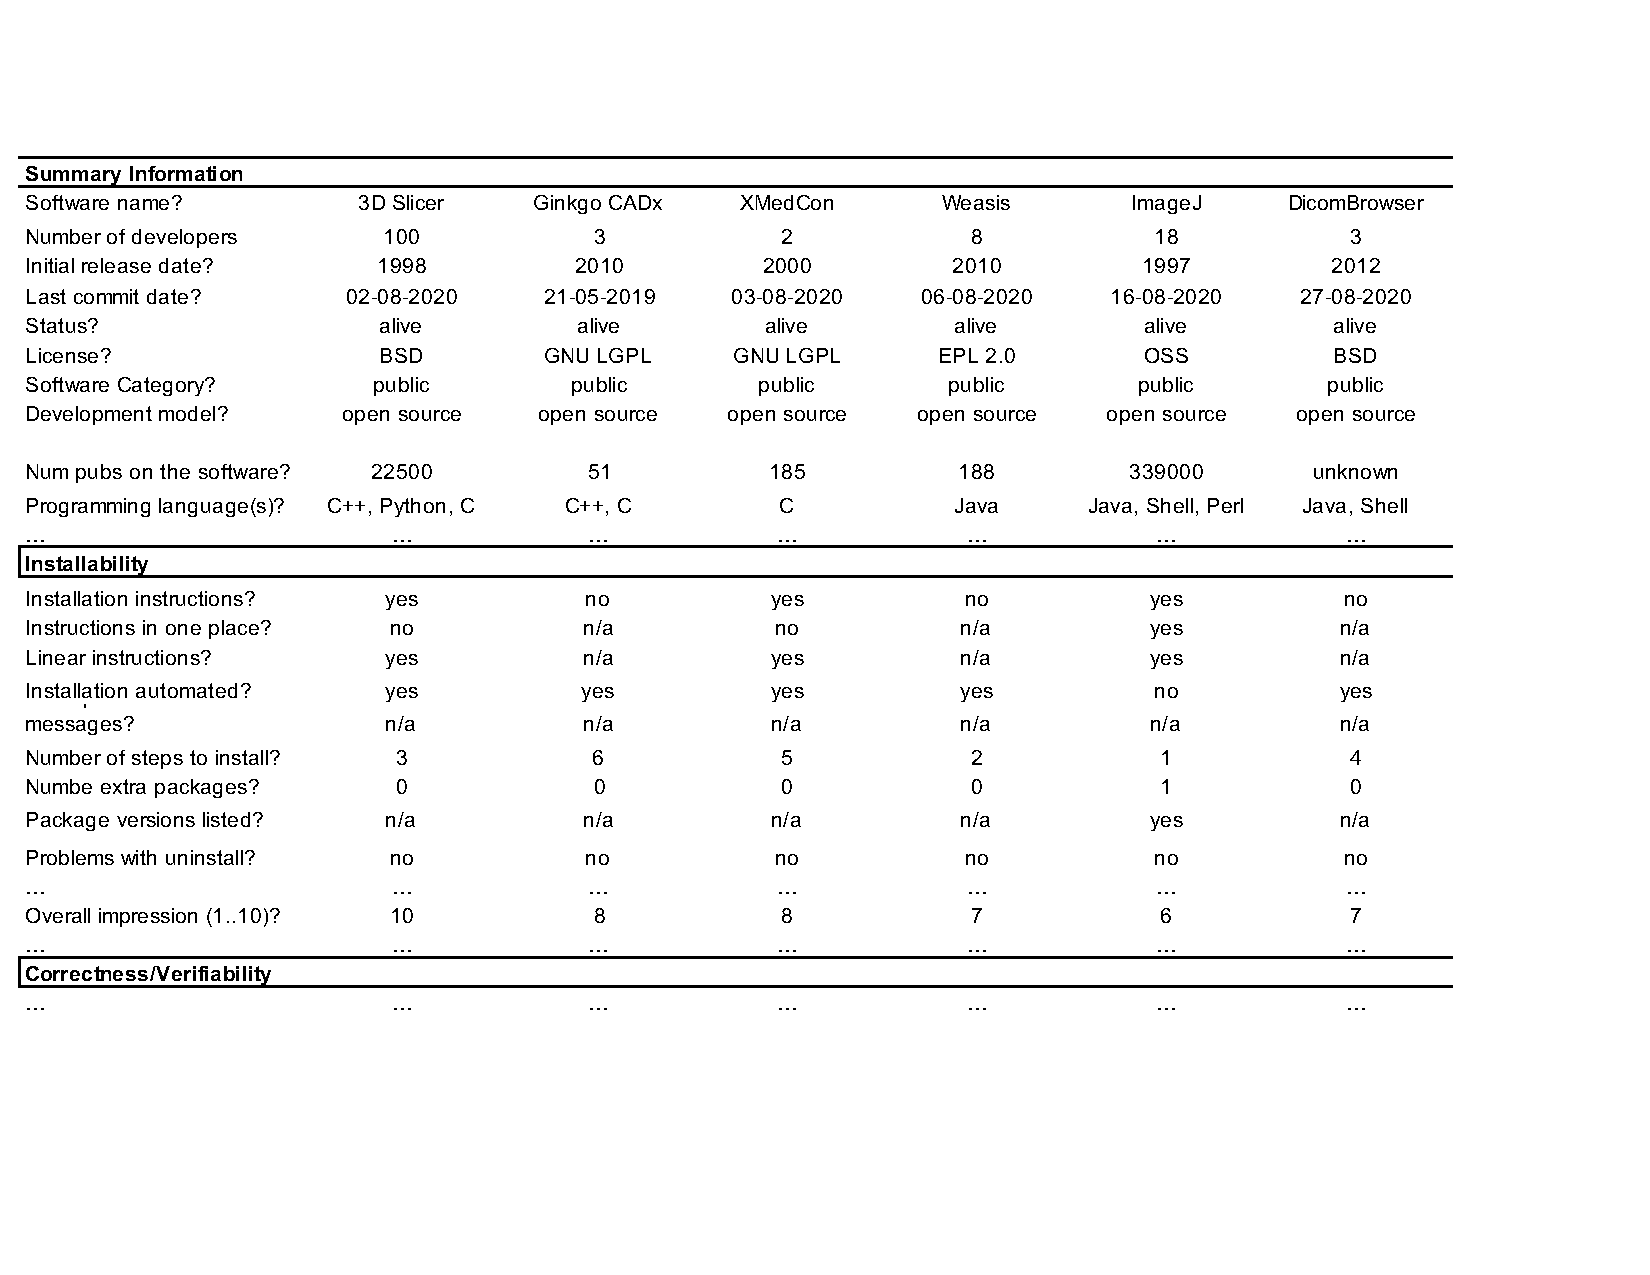
\includegraphics[scale=0.67]{template.pdf}
\caption{Grading template example}
\label{fg_grading_template_example}
\end{figure*}

The full template consists of 108 questions over 9 qualities.  These
questions are designed to be unambiguous, quantifiable, and measurable
with constrained time and domain knowledge.

The grader, after answering questions for each quality assigns an overall
score (between 1 and 10) based on the answers.  Several of the qualities use
the word ``surface'' to highlight that these particular qualities are a shallow
measure.  For example, usability is not measured using user studies.
Instead, we look for signs that the developers considered usability.
We use two freeware tools to collect repository related data:
\href{https://github.com/tomgi/git_stats}{GitStats} and
\href{https://github.com/boyter/scc}{Sloc Cloc and Code (scc)}.  Further
details on quality measurement are provided in [redacted for double blind].
%% DOUBLE BLIND
%Smith et al.\ (2024) \cite{SmithEtAl2024_MI_SOP}.

\subsubsection{Analytic Hierarchy Process (AHP)} \label{sec_AHP}

Developed by Saaty in the 1970s, AHP is widely used to analyze multiple criteria
decisions~\cite{VaidyaEtAl2006}. AHP organizes multiple criteria in a
hierarchical structure and uses pairwise comparisons between alternatives to
calculate relative ratios~\cite{Saaty1990}. AHP works with sets of $n$
\textit{options} and $m$ \textit{criteria}.  In our project $n=29$ and $m=9$
since there are 29 options (software products) and 9 criteria (qualities). With
AHP the sum of the grades (scores) for all products for a given quality will be
1.0.  We rank the software for each of the qualities, and then we combine the
quality rankings into an overall ranking based on the relative priorities
between qualities.

\subsubsection{Interview Methods} \label{sec_interview_methods}

The repository-based measurements are incomplete because they don't generally
capture the development process, the developer pain points, the perceived
threats to software quality, and the developers' strategies to address these
threats.  Therefore, part of our methodology involves interviewing developers.
We based our interviews on a list of 20 questions, which can be found in
[citation redacted for double blind].
%Smith et al. \cite{SmithEtAl2021}. 
Some questions are about the background of the software, the development teams,
the interviewees, and how they organize their projects.  We also ask about the
developer's understanding of the users. Additional questions focus on the current and
past difficulties, and the solutions the team has found, or plan to try. We also
discuss documentation, both with respect to how it is currently done, and how it
is perceived. A few questions are about specific software qualities, such as
maintainability, understandability, usability, and reproducibility. The
interviews are semi-structured based on the question list.

\section{In-Scope Open-Source MI Software} \label{SecWhatProjects}

We initially identified 48 candidate software projects from the literature
\cite{Bjorn2017, Bruhschwein2019, Haak2015}, on-line articles \cite{Emms2019,
Hasan2020, Mu2019}, and forum discussions \cite{Samala2014}.  Then we filtered
as follows:

\begin{enumerate}

\item Removed the packages with no source code available, such as
\textit{MicroDicom}, \textit{Aliza}, and \textit{jivex}.

\item Focused on MI software that provides visualization functions.  We removed
seven packages that were toolkits or libraries, such as \textit{VTK},
\textit{ITK}, and \textit{dcm4che}, and another three that were for PACS.

\item Removed \textit{Open Dicom Viewer} as it has not received any
updates since 2011.

\end{enumerate}

The Domain Expert provided a list 12 software packages.  We found 6 packages
were on both lists: \textit{3D Slicer}, \textit{Horos}, \textit{ImageJ},
\textit{Fiji}, \textit{MRIcron} (we use its descendant \textit{MRIcroGL}) and
\textit{Mango} (we use the web version \textit{Papaya}).  The remaining six
packages were on our out-of-scope list. The Domain Expert agreed with our final
choice of 29 packages.  Table~\ref{tab_final_list} summarizes the in-scope
open-source MI software that is available at the time of measurement (the year
2020), thus answering \rqref{RQ_WhatProjects}.

\begin{table*}[ht!]
\centering
\begin{tabular}{p{3.7cm}lllllllll}
\toprule
\multirow{2}{*}{Software} & \multirow{2}{*}{Rlsd} & \multirow{2}{*}{Updated} & \multirow{2}{*}{Fnd} & \multirow{2}{*}{NOC} & \multirow{2}{*}{LOC} & \multicolumn{3}{c}{OS} & \multirow{2}{*}{Web} \\ \cmidrule{7-9}
 &  &  &  &  &  & W & M & L &  \\ \midrule
ParaView \cite{Ahrens2005} & 2002 & 2020-10 & \checkmark & 100 & 886326 & \checkmark & \checkmark & \checkmark & \checkmark \\
Gwyddion \cite{Nevcas2012} & 2004 & 2020-11 &  & 38 & 643427 & \checkmark & \checkmark & \checkmark &  \\
Horos \cite{horosproject2020} & ? & 2020-04 &  & 21 & 561617 &  & \checkmark &  &  \\
OsiriX Lite \cite{PixmeoSARL2019} & 2004 & 2019-11 &  & 9 & 544304 &  & \checkmark &  &  \\
3D Slicer \cite{Kikinis2014} & 1998 & 2020-08 & \checkmark & 100 & 501451 & \checkmark & \checkmark & \checkmark &  \\
Drishti \cite{Limaye2012} & 2012 & 2020-08 &  & 1 & 268168 & \checkmark & \checkmark & \checkmark &  \\
Ginkgo CADx \cite{Wollny2020} & 2010 & 2019-05 &  & 3 & 257144 & \checkmark & \checkmark & \checkmark &  \\
GATE \cite{Jan2004} & 2011 & 2020-10 &  & 45 & 207122 &  & \checkmark & \checkmark &  \\
3DimViewer \cite{TESCAN2020} & ? & 2020-03 & \checkmark & 3 & 178065 & \checkmark & \checkmark &  &  \\
medInria \cite{Fillard2012} & 2009 & 2020-11 &  & 21 & 148924 & \checkmark & \checkmark & \checkmark &  \\
BioImage Suite Web \cite{Papademetris2005} & 2018 & 2020-10 & \checkmark & 13 & 139699 &
\checkmark & \checkmark & \checkmark & \checkmark \\
Weasis \cite{Roduit2021} & 2010 & 2020-08 &  & 8 & 123272 & \checkmark & \checkmark & \checkmark &  \\
AMIDE \cite{Loening2017} & 2006 & 2017-01 &  & 4 & 102827 & \checkmark & \checkmark & \checkmark &  \\
XMedCon \cite{Nolf2003} & 2000 & 2020-08 &  & 2 & 96767 & \checkmark & \checkmark & \checkmark &  \\
ITK-SNAP \cite{Yushkevich2006} & 2006 & 2020-06 & \checkmark & 13 & 88530 & \checkmark & \checkmark & \checkmark &  \\
Papaya \cite{UTHSCSA2019} & 2012 & 2019-05 &  & 9 & 71831 & \checkmark & \checkmark & \checkmark &  \\
OHIF Viewer \cite{Ziegler2020} & 2015 & 2020-10 &  & 76 & 63951 & \checkmark & \checkmark & \checkmark & \checkmark \\
SMILI \cite{Chandra2018} & 2014 & 2020-06 &  & 9 & 62626 & \checkmark & \checkmark & \checkmark &  \\
INVESALIUS 3 \cite{Amorim2015} & 2009 & 2020-09 &  & 10 & 48605 & \checkmark & \checkmark & \checkmark &  \\
dwv \cite{Martelli2021} & 2012 & 2020-09 &  & 22 & 47815 & \checkmark & \checkmark & \checkmark & \checkmark \\
DICOM Viewer \cite{Afsar2021} & 2018 & 2020-04 & \checkmark & 5 & 30761 & \checkmark & \checkmark & \checkmark &  \\
MicroView \cite{ParallaxInnovations2020} & 2015 & 2020-08 &  & 2 & 27470 & \checkmark & \checkmark & \checkmark &  \\
MatrixUser \cite{Liu2016} & 2013 & 2018-07 &  & 1 & 23121 & \checkmark & \checkmark & \checkmark &  \\
Slice:Drop \cite{Haehn2013} & 2012 & 2020-04 &  & 3 & 19020 & \checkmark & \checkmark & \checkmark & \checkmark \\
dicompyler \cite{Panchal2010} & 2009 & 2020-01 &  & 2 & 15941 & \checkmark & \checkmark &  &  \\
Fiji \cite{Schindelin2012} & 2011 & 2020-08 & \checkmark & 55 & 10833 & \checkmark & \checkmark & \checkmark &  \\
ImageJ \cite{Rueden2017} & 1997 & 2020-08 & \checkmark & 18 & 9681 & \checkmark & \checkmark & \checkmark &  \\
MRIcroGL \cite{Rorden2021} & 2015 & 2020-08 &  & 2 & 8493 & \checkmark & \checkmark & \checkmark &  \\
DicomBrowser \cite{Archie2012} & 2012 & 2020-08 &  & 3 & 5505 & \checkmark & \checkmark & \checkmark &  \\ \bottomrule
\end{tabular}
\caption{Final software list (sorted in descending order of the number of Lines
Of Code (LOC))}
\label{tab_final_list}
\end{table*}

In Table~\ref{tab_final_list} the projects are sorted in descending order of
lines of code.  We found the initial release dates (Rlsd) for most projects and
marked the two unknown dates with ``?''. The date of the last update is the date
of the latest update, at the time of measurement. We found funding information
(Fnd) for only eight projects.  For the Number Of Contributors (NOC) we
considered anyone who made at least one accepted commit as a contributor. The
NOC is not usually the same as the number of long-term project members, since
many projects received change requests and code from the community.  With
respect to the OS, 25 packages work on all three OSs: Windows (W), macOS (M),
and Linux (L). Although the usual approach to cross-platform compatibility was
to work natively on multiple OSes, five projects achieved platform-independence
via web applications. The full measurement data for all packages is available on
[removed for blind review]
%\href{https://data.mendeley.com/datasets/k3pcdvdzj2/1} {Mendeley Data}.  
%% DOUBLE BLIND

The programming languages used in order of decreasing popularity are \CC,
JavaScript, Java, C, Python, Pascal, Matlab.  The most popular language is \CC,
for 11 of 29 projects; Pascal and Matlab were each used for a single project.

\section{Which Projects Follow Best Practices?} \label{SecMeasurementResults}

We measured the software as described in
Section~\ref{SecMethodology}.  In the absence of a specific real world context,
we assumed all nine qualities are equally important.
Figure~\ref{fg_overall_scores} shows the overall AHP scores in descending order.

\begin{figure*}[ht!]
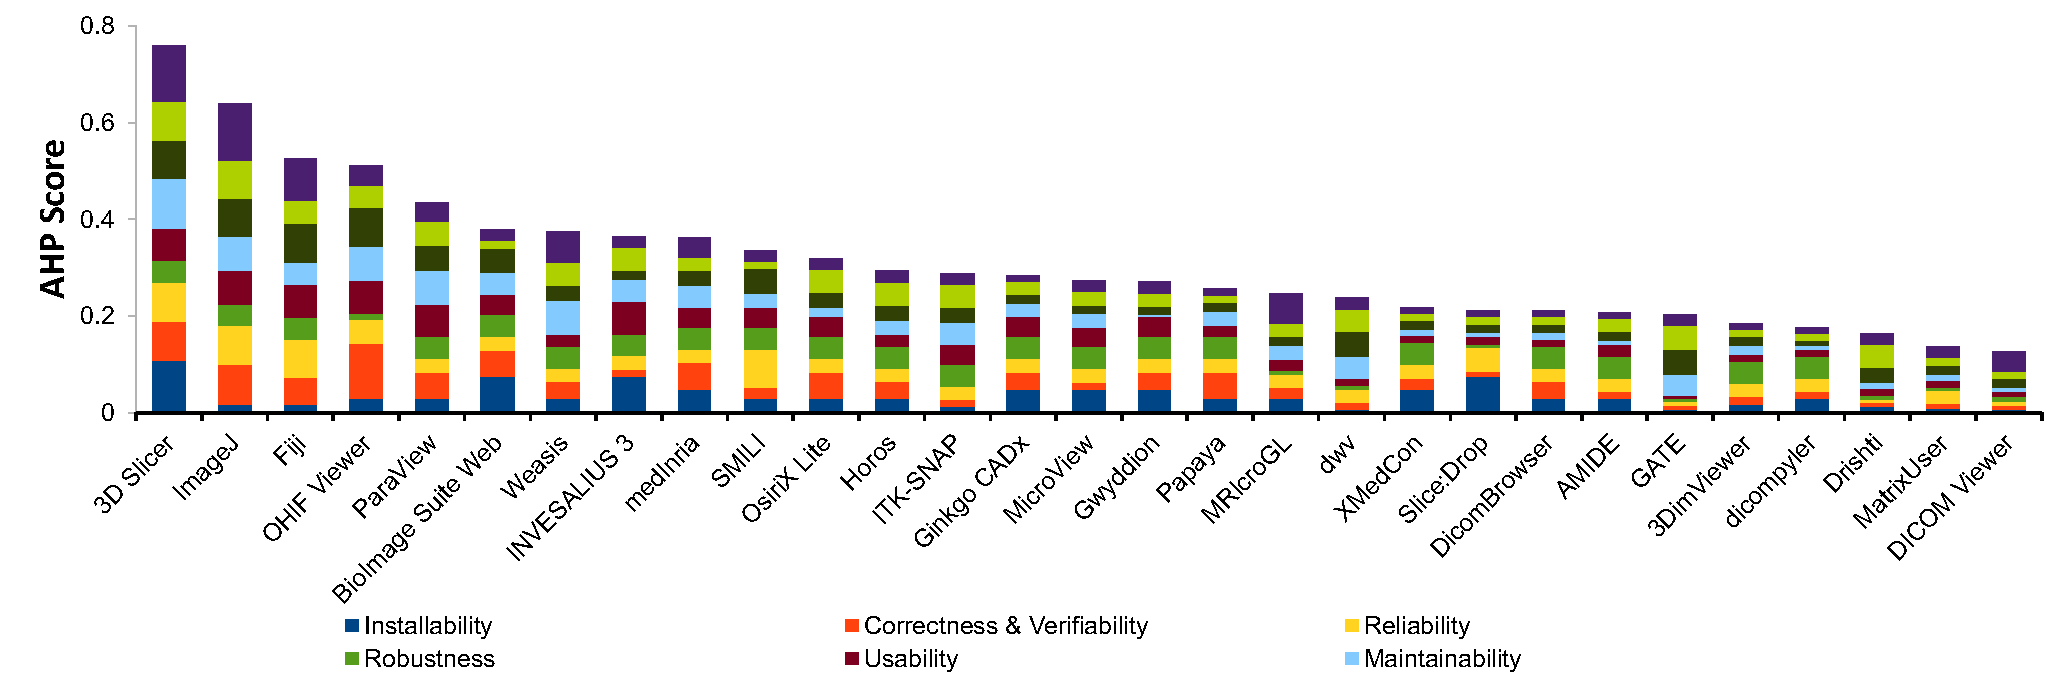
\includegraphics[scale=0.47]{overall_scores.pdf}
\caption{Overall AHP scores with an equal weighting for all 9 software qualities}

\label{fg_overall_scores}
\end{figure*}

The top four software products \textit{3D Slicer}, \textit{ImageJ},
\textit{Fiji}, and \textit{OHIF Viewer} have higher scores in most criteria.
\textit{3D Slicer} has a score in the top two for all qualities; \textit{ImageJ}
ranks near the top for all qualities, except for correctness \& verifiability.
\textit{OHIF Viewer} and \textit{Fiji} have similar overall scores, with
\textit{Fiji} doing better in installability and \textit{OHIF Viewer} doing
better in correctness \& verifiability.  Given the installation problems, we may
have underestimated the scores on reliability and robustness for \textit{DICOM
Viewer}, but we compared it equally for the other qualities.

The overall score is based on the measurement of the identified qualities. Full
details of how the projects compare for each quality can be found in [citation
redacted for blind review].
%% DOUBLE BLIND
%Smith et al.~\cite{SmithEtAl2024_MI_SOP}
The highlights are as follows:

\begin{description}

\item [Installability] We found installation instructions for 16 projects, but
two did not need them (\textit{BioImage Suite Web} and \textit{Slice:Drop}) as
they are web applications. 10 of the projects required extra dependencies: Five
depend on a specific browser; \textit{dwv}, \textit{OHIF Viewer}, and
\textit{GATE} needs extra libraries to build; \textit{ImageJ} and \textit{Fiji}
need an unzip tool; \textit{MatrixUser} needs Matlab; \textit{DICOM Viewer}
needs a Nextcloud platform. We were not able to install \textit{GATE},
\textit{dwv}, \textit{DICOM Viewer} even after trying for 2 hours (each).

\item [Correctness \& Verifiability] The packages with higher scores for
correctness and verifiability used a wider array of techniques to improve
correctness, and had better documentation to support this. For instance, we
looked for evidence of unit testing, and found evidence for only about half of
the projects. We identified five projects using continuous integration tools:
\textit{3D Slicer}, \textit{ImageJ}, \textit{Fiji}, \textit{dwv}, and
\textit{OHIF Viewer}. The only requirements-related document we found was a road
map of \textit{3D Slicer}, which contained design requirements for upcoming
changes.

\item [Surface Reliability] We were able to follow the steps in the tutorials
that existed (seven packages had them.) However, \textit{GATE} could not open
macro files and became unresponsive several times, without any descriptive error
message. We found that \textit{Drishti} crashed when loading damaged image
files, without showing any descriptive error message.

\item [Surface Robustness] According to their documentation, all 29 software
packages should support the DICOM standard. To test robustness, we prepared two
types of image files: correct and incorrect formats (with the incorrect format
created by relabelling a text file to have the ``.dcm'' extension).  All
software packages loaded the correct format image, except for \textit{GATE},
which failed for unknown reasons.  For the broken format, \textit{MatrixUser},
\textit{dwv}, and \textit{Slice:Drop} ignored the incorrect format, did not show
any error message and displayed a blank image.  \textit{MRIcroGL} behaved
similarly except that it showed a meaningless image.  \textit{Drishti}
successfully detected the broken format, but the software then crashed.

\item [Surface Usability] The software with higher usability scores usually
provided both comprehensive documented guidance and a good user experience.
\textit{INVESALIUS 3} provided an excellent example of a detailed and precise
user manual. \textit{GATE} also provided numerous documents, but unfortunately
we had difficulty understanding and using them. We found getting started
tutorials for only 11 projects, but a user manual for 22 projects.
\textit{MRIcroGL} was the only project that explicitly documented expected user
characteristics.

\item [Maintainability] We gave \textit{3D Slicer} the highest score for
maintainability because we found it had the most comprehensive artifacts. Only a
few of the 29 projects had a product, developer's manual, or API (Application
Programming Interface) documentation, and only \textit{3D Slicer},
\textit{ImageJ}, \textit{Fiji} included all three documents.  Moreover,
\textit{3D Slicer} has a much higher percentage of closed issues (92\%) compared
to \textit{ImageJ} (52\%) and \textit{Fiji} (64\%). Twenty-seven of the 29
projects used git for version control, with 24 of these using GitHub.
\textit{AMIDE} used Mercurial and \textit{Gwyddion} used Subversion.
\textit{XMedCon}, \textit{AMIDE}, and \textit{Gwyddion} used SourceForge.
\textit{DicomBrowser} and \textit{3DimViewer} used BitBucket. 

\item [Reusability] We have assumed that smaller code files are
likely more reusable -- see Table \ref{tab_loc_per_file} for the details.

\item [Surface Understandability] All projects had a consistent coding style
with parameters in the same order for all functions, modularized code, and,
clear comments that indicate what is done, not how. However, we only found
explicit identification of a coding standard for 3 out of the 29: \textit{3D
Slicer}, \textit{Weasis}, and \textit{ImageJ}. We also found hard-coded
constants (rather than symbolic constants) in \textit{medInria},
\textit{dicompyler}, \textit{MicroView}, and \textit{Papaya}. We did not find
any reference to the algorithms used in projects \textit{XMedCon},
\textit{DicomBrowser}, \textit{3DimViewer}, \textit{BioImage Suite Web},
\textit{Slice:Drop}, \textit{MatrixUser}, \textit{DICOM Viewer},
\textit{dicompyler}, and \textit{Papaya}. 

\item [Visibility/Transparency] Generally speaking, the teams that actively
documented their development process and plans scored higher.  \textit{3D
Slicer} and \textit{ImageJ} were the only projects to include documentation for
all of the following: development process, project status, development
environment and release notes.

\end{description}  

\begin{table*}[ht!]
\centering
\begin{tabular}{lllll}
\toprule
\multirow{2}{*}{Software} & \multirow{2}{*}{Text Files} & \multirow{2}{*}{Total Lines} & \multirow{2}{*}{LOC} & \multirow{2}{*}{LOC/file} \\
 &  &  &  &  \\ 
\midrule
OHIF Viewer & 1162 & 86306 & 63951 & 55 \\
3D Slicer & 3386 & 709143 & 501451 & 148 \\
Gwyddion & 2060 & 787966 & 643427 & 312 \\
ParaView & 5556 & 1276863 & 886326 & 160 \\
OsiriX Lite & 2270 & 873025 & 544304 & 240 \\
Horos & 2346 & 912496 & 561617 & 239 \\
medInria & 1678 & 214607 & 148924 & 89 \\
Weasis & 1027 & 156551 & 123272 & 120 \\
BioImage Suite Web & 931 & 203810 & 139699 & 150 \\
GATE & 1720 & 311703 & 207122 & 120 \\
Ginkgo CADx & 974 & 361207 & 257144 & 264 \\
SMILI & 275 & 90146 & 62626 & 228 \\
Fiji & 136 & 13764 & 10833 & 80 \\
Drishti & 757 & 345225 & 268168 & 354 \\
ITK-SNAP & 677 & 139880 & 88530 & 131 \\
3DimViewer & 730 & 240627 & 178065 & 244 \\
DICOM Viewer & 302 & 34701 & 30761 & 102 \\
ImageJ & 40 & 10740 & 9681 & 242 \\
dwv & 188 & 71099 & 47815 & 254 \\
MatrixUser & 216 & 31336 & 23121 & 107 \\
INVESALIUS 3 & 156 & 59328 & 48605 & 312 \\
AMIDE & 183 & 139658 & 102827 & 562 \\
Papaya & 110 & 95594 & 71831 & 653 \\
MicroView & 137 & 36173 & 27470 & 201 \\
XMedCon & 202 & 129991 & 96767 & 479 \\
MRIcroGL & 97 & 50445 & 8493 & 88 \\
Slice:Drop & 77 & 25720 & 19020 & 247 \\
DicomBrowser & 54 & 7375 & 5505 & 102 \\
dicompyler & 48 & 19201 & 15941 & 332 \\ 
\bottomrule
\end{tabular}
\caption{Number of files and lines (by reusability scores)}
\label{tab_loc_per_file}
\end{table*}

\section{Comparison to Community Ranking} \label{Sec_VsCommunityRanking}

We use GitHub stars, number of forks and
number of people watching the projects as proxies for community ranking.
Table~\ref{tab_ranking_vs_GitHub} show the statistics for data collected in July
2021.

Our ranking and GitHub popularity, at least for the top five projects, seems to
line up well. However, we ranked some popular packages fairly low, such
as \textit{dwv}. This is because we were unable to build it locally, even though
we followed its installation instructions. However, we were able to use its web
version for the rest of the measurements. Additionally, this version did not
detect a broken DICOM file and instead displayed a blank image
(Section~\ref{SecMeasurementResults}).  \textit{DICOM Viewer} ranked low as we
were unable to install the NextCloud platform.

We weighted all qualities equally, which is not the likely the same weighting
that users implicitly use. To properly assess this would require a broad user
study.  Furthermore our measures of popularity (like stars) are only \emph{proxies} which
are biased towards past rather than current preferences~\cite{Szulik2017}, as
these are monotonically increasing quantities. Finally there are often more
factors than just quality that influence the popularity of 
products.

\begingroup
\renewcommand{\arraystretch}{0.85}
\begin{table*}[ht!]
\centering
\begin{tabular}{llllll}
\toprule
Software & Comm.\ Rank & Our Rank & Stars/yr & Watches/yr & Forks/yr \\ 
\midrule
3D Slicer & 1 & 1 & 284 & 19 & 128 \\
OHIF Viewer & 2 & 4 & 277 & 19 & 224 \\
dwv & 3 & 19 & 124 & 12 & 51 \\
ImageJ & 4 & 2 & 84 & 9 & 30 \\
ParaView & 5 & 5 & 67 & 7 & 28 \\
Horos & 6 & 12 & 49 & 9 & 18 \\
Papaya & 7 & 17 & 45 & 5 & 20 \\
Fiji & 8 & 3 & 44 & 5 & 21 \\
DICOM Viewer & 9 & 29 & 43 & 6 & 9 \\
INVESALIUS 3 & 10 & 8 & 40 & 4 & 17 \\
Weasis & 11 & 7 & 36 & 5 & 19 \\
dicompyler & 12 & 26 & 35 & 5 & 14 \\
OsiriX Lite & 13 & 11 & 34 & 9 & 24 \\
MRIcroGL & 14 & 18 & 24 & 3 & 3 \\
GATE & 15 & 24 & 19 & 6 & 26 \\
Ginkgo CADx & 16 & 14 & 19 & 4 & 6 \\
BioImage Suite Web & 17 & 6 & 18 & 5 & 7 \\
Drishti & 18 & 27 & 16 & 4 & 4 \\
Slice:Drop & 19 & 21 & 10 & 2 & 5 \\
ITK-SNAP & 20 & 13 & 9 & 1 & 4 \\
medInria & 21 & 9 & 7 & 3 & 6 \\
SMILI & 22 & 10 & 3 & 1 & 2 \\
MatrixUser & 23 & 28 & 2 & 0 & 0 \\
MicroView & 24 & 15 & 1 & 1 & 1 \\
Gwyddion & 25 & 16 & n/a & n/a & n/a \\
XMedCon & 26 & 20 & n/a & n/a & n/a \\
DicomBrowser & 27 & 22 & n/a & n/a & n/a \\
AMIDE & 28 & 23 & n/a & n/a & n/a \\
3DimViewer & 29 & 25 & n/a & n/a & n/a \\ 
\bottomrule
\end{tabular}
\caption{Software ranking by our methodology versus the community (Comm.)\
ranking using GitHub metrics (Sorted in descending order of community
popularity, as estimated by the number of new stars per year)}
\label{tab_ranking_vs_GitHub}
\end{table*}
\endgroup

Although both rankings are imperfect measures, they nevertheless suggest a
correlation between best practices and popularity. We don't know if this is
causal, in either direction (i.e. if best practices enable popularity or if
popularity increases the need for best practices).

\section{Comparing with Recommended Software Artifacts} \label{Sec_CompareArtifacts}

We use a set of nine research software development
guidelines to compare recommended software artifacts versus those present in MI
software:
\begin{itemize}
\item United States Geological Survey Software Planning Checklist
\cite{USGS2019},
\item DLR (German Aerospace Centre) Software Engineering Guidelines
\cite{TobiasEtAl2018}, 
\item Scottish Covid-19 Response Consortium Software Checklist
\cite{BrettEtAl2021},
\item Good Enough Practices in Scientific Computing \cite{WilsonEtAl2016},
\item xSDK (Extreme-scale Scientific Software Development Kit) Community Package
Policies \cite{SmithAndRoscoe2018},
\item Trilinos Developers Guide \cite{HerouxEtAl2008},
\item EURISE (European Research Infrastructure Software Engineers') Network
Technical Reference \cite{ThielEtAl2020},
\item CLARIAH (Common Lab Research Infrastructure for the Arts and Humanities)
Guidelines for Software Quality \cite{vanGompelEtAl2016}, and
\item A Set of Common Software Quality Assurance Baseline Criteria for Research
Projects \cite{OrvizEtAl2017}.
\end{itemize}

\begin{table*}[ht!]
\begin{center}
\begin{tabular}{ p{3.5cm}p{0.5cm}p{0.5cm}p{0.5cm}p{0.5cm}p{0.5cm}p{0.5cm}p{0.5cm}p{0.5cm}p{0.5cm}p{0.5cm} }
\toprule
~ \ & \cite{USGS2019} & \cite{TobiasEtAl2018} & \cite{BrettEtAl2021} &
\cite{WilsonEtAl2016} & \cite{SmithAndRoscoe2018} & \cite{HerouxEtAl2008} &
\cite{ThielEtAl2020} & \cite{vanGompelEtAl2016} & \cite{OrvizEtAl2017} & MI\\
\midrule
LICENSE & \checkmark & \checkmark & \checkmark & \checkmark & \checkmark & &
\checkmark & \checkmark & \checkmark & C\\
README &  & \checkmark & \checkmark & \checkmark & \checkmark & & \checkmark &
\checkmark & \checkmark & C\\
CONTRIBUTING &  & \checkmark & \checkmark & \checkmark & \checkmark & &
\checkmark & \checkmark & \checkmark & R\\
CITATION &  &  &  & \checkmark & & & & \checkmark & \checkmark & U\\
CHANGELOG &  & \checkmark &  & \checkmark & \checkmark & & \checkmark &  &  & U\\
INSTALL &  &  &  &  & \checkmark & & \checkmark & \checkmark & \checkmark & U\\
\midrule
Uninstall &  &  &  &  & & & & \checkmark & &  \\
Dependency List &  &  & \checkmark & & \checkmark & & & \checkmark &  & R\\
Authors &  &  &  &  &  &  & \checkmark & \checkmark & \checkmark & U\\
Code of Conduct &  &  &  &  & & & \checkmark & & & R\\
Acknowledgements &  &  &  &  &  &  & \checkmark & \checkmark & \checkmark & U\\
Code Style Guide &  & \checkmark &  &  & & & \checkmark & \checkmark & \checkmark & R\\
Release Info. &  & \checkmark &  &  & & \checkmark & \checkmark & & & C\\
Prod.\ Roadmap &  &  &  &  & & \checkmark & \checkmark & \checkmark & & R\\
\midrule
Getting started &  &  &  &  & \checkmark & & \checkmark & \checkmark & \checkmark & R\\
User manual &  &  & \checkmark &  & & & \checkmark & & & C\\
Tutorials &  &  &  &  & & & \checkmark & & & U\\
FAQ &  &  &  &  & & & \checkmark & \checkmark & \checkmark & U\\
\midrule
Issue Track &  & \checkmark & \checkmark & & \checkmark & \checkmark &
\checkmark & & \checkmark & C\\
Version Control &  & \checkmark & \checkmark & \checkmark & \checkmark &
\checkmark & \checkmark & \checkmark & \checkmark & C\\ 
Build Scripts &  & \checkmark &  & \checkmark & \checkmark & \checkmark &
\checkmark & & \checkmark & U\\
\midrule
Requirements &  & \checkmark &  &  & & \checkmark &  &  & \checkmark & R\\
Design Doc.\ &  & \checkmark  & \checkmark &  & \checkmark & & \checkmark &
\checkmark& \checkmark & R\\
API Doc. &  &  &  &  & \checkmark & & \checkmark & \checkmark & \checkmark & R\\
Test Plan &  & \checkmark &  &  & & \checkmark & & & &  \\
Test Cases & \checkmark & \checkmark & \checkmark &  & \checkmark & \checkmark &
\checkmark & \checkmark & \checkmark & U\\
\bottomrule
\end{tabular}
\caption{Comparison of Recommended Artifacts in Software Development Guidelines
to Artifacts in MI Projects (C for Common, U for Uncommon and R for Rare)}
\label{Tbl_Guidelines}
\end{center}
\end{table*}

We show the recommended artifacts in Table~\ref{Tbl_Guidelines}, one per row.
For a given row, a checkmark in one of the columns means that the corresponding
guideline recommends this artifact.  The last column shows whether the artifact
appears in the measured set of MI software, either not at all (blank), commonly
(C) (20 to 29 ($>$67\%) packages), uncommonly (U) (10 to 19 (33-67\%) packages)
or rarely (R) (1 to 9 ($<$33\%) packages).  We did our best to interpret the
meaning of each artifact consistently between guidelines and specific MI
software, but the terminology and the contents of artifacts are not
standardized.  The challenge even exists for the ubiquitous README file.  The
content of README files shows significant variation between
projects~\cite{PranaEtAl2018}.  Some content is reasonably consistent, with 97\%
of README files contain at least one section describing the `What' of the
repository and 89\% offering some `How' content, other categories are more
variable.  For instance, information on `Contribution', `Why', and `Who', appear
in 28\%, 26\% and 53\% of the analyzed files, respectively~\cite{PranaEtAl2018}.  

\begin{table*}[ht!]
    \begin{center}
    \begin{tabular}{ p{3.8 cm} p{6.4 cm} p{4.5 cm}}
    \toprule
    Common & Uncommon & Rare \\
    \midrule
    README (29) & Build scripts (18) & Getting Started (9)\\
    Version control (29) & Tutorials (18) & Developer's manual (8)\\
    License (28) & Installation guide (16) & Contributing (8)\\
    Issue tracker (28) & Test cases (15) & API documentation (7)\\
    User manual (22) & Authors (14) & Dependency list (7)\\
    Release info. (22) & Frequently Asked Questions (14) & Troubleshooting guide (6)\\
     & Acknowledgements (12) & Product roadmap (5)\\
     & Changelog (12) & Design documentation (5)\\
     & Citation (11) & Code style guide (3)\\
     & & Code of conduct (1)\\
     & & Requirements (1)\\
    \bottomrule
    \end{tabular}
    \caption{Artifacts Present in MI Packages, Classified by Frequency
    (number of occurrences)}
    \label{artifactspresent}
    \end{center}
\end{table*}

Popularity in Table~\ref{Tbl_Guidelines} does not imply that these oft
recommended artifacts are the most important. Guidelines are often brief, to
encourage adoption, and thus even guidelines that mention the need for
installation instructions rarely mention uninstallation instructions.  Two items
in Table~\ref{artifactspresent}, which presents our measurements for the MI
software, do not appear in any guidelines: \emph{Troubleshooting guide} and
\emph{Developer's manual}.  However the information within these documents
overlaps with the recommended artifacts.  Troubleshooting information often can
be found in a User Manual, while the information in a ``Developer's Manual'' is
often scattered amongst many other documents.

Three of the 26 recommended artifacts were never observed in the MI software:
i) Uninstall, ii) Test plans, and iii) Requirements. It is possible that
some of these were created but never put under version control.

Neglecting requirements documentation is unfortunately common for research
software, and MI software is no exception to this trend.  Although such
documentation is recommended by some \cite{TobiasEtAl2018, HerouxEtAl2008,
SmithAndKoothoor2016}, in practice this is rare~\cite{HeatonAndCarver2015}.
Sanders and Kelly \cite{SandersAndKelly2008} interviewed 16 scientists from 10
disciplines and found that none of the scientists created requirements
specifications, unless regulations in their field mandated such a document.
Requirements are the least commonly produced type of documentation for research
software in general \cite{Nguyen-HoanEtAl2010}. 

This is unfortunate as when scientific developers are surveyed on their pain
points, Wiese et al.~\cite{WieseEtAl2019} found that software requirements and
management is the software engineering discipline that most hurts them,
accounting for 23\% of the technical problems reported by study participants.
Further adding to the misfortune, there is a widespread perception that up-front
requirements are impossible for research software \cite{CarverEtAl2007,
SegalAndMorris2008}. Fortunately an iterative approach to requirements is
feasible~\cite{Smith2016}, and research-software specific templates
exist~\cite{SmithEtAl2007}. 

A theme emerges amongst the artifacts rarely observed in practice: they
are developer-focused (a list of library dependencies, a contributor's guide,
a developer Code of Conduct, coding style guidelines, product roadmap, design
documentation and API documentation).

Other communities use checklists to help with best practices. Examples include
checklists for merging branches~\cite{Brown2015}, for saving and sharing changes
to the project~\cite{WilsonEtAl2016}, for new and departing team
members~\cite{HerouxAndBernholdt2018}, for processes related to commits and
releases~\cite{HerouxEtAl2008} and for overall software
quality~\cite{ThielEtAl2020, SSI2022}.

MI projects fall somewhat short of recommended best practices, but are not alone
amongst research software projects. This gap has been documented
before~\cite{Storer2017,JohansonAndHasselbring2018}, and is known to cause
sustainability and reliability problems \cite{FaulkEtAl2009}, and to waste
development effort~\cite{deSouzaEtAl2019}.

\section{Comparison of Tool Usage Between MI and Other Research Software}
\label{Sec_CompareTools}

We use data from interviews, as described in Section~\ref{sec_interview_methods}
to answer \rqref{RQ_CompareToolsProjMngmnt} (tool usage),
\rqref{RQ_CompareMethodologies} (methodology) and \rqref{RQ_PainPoints} (pain
points). Requests were sent to all 29 projects.  Nine developers from eight of
the projects agreed to participate: \textit{3D Slicer}, \textit{INVESALIUS 3},
\textit{dwv}, \textit{BioImage Suite Web}, \textit{ITK-SNAP},
\textit{MRIcroGL}, \textit{Weasis}, and \textit{OHIF}. We spent about 90
minutes for each interview. The full interview answers can be
found in [citation redacted for blind review].
%\cite{Dong2021}.

Developers use software tools for user support, version control,
Continuous Integration and Deployment (CI/CD), documentation and project
management.  We summarize the tool usage in each of these categories, and
compare this to the usage by the research software community.

\paragraph{User support} Table~\ref{tab_user_support_model} summarizes the user
support models by the number of projects using each model (projects may use
more than one support model).

\begin{table}[ht!]
\centering
\begin{tabular}{lc}
\toprule
\multicolumn{1}{c}{User Support Model} & Num.\ Projects \\
\midrule
GitHub issue & 24 \\
Frequently Asked Questions (FAQ) & 12 \\
Forum & 10 \\
E-mail address & 9 \\
GitLab issue, SourceForge discussions & 2 \\
Troubleshooting & 2 \\
Contact form & 1 \\ 
\bottomrule
\end{tabular}
\caption{\label{tab_user_support_model}User support models by number of projects}
\end{table}

\paragraph{Version control} Most teams interviewed (eight of nine) use GitHub
for version control, which makes it unsurprising that they also use pull
requests for managing community contributions. The experience of using GitHub
was reported as generally positive; some teams had actively migrated to GitHub
from other version control systems.  This represents a considerable uptake since
its rare use in 2006~\cite{Wilson2006}, which matches the uptake in other
communities: 10 years ago Nguyen et al~\cite{Nguyen-HoanEtAl2010} estimated that
only 50\% of research software projects used version control, and by 2018 this
had jumped to over 80\%~\cite{AlNoamanyAndBorghi2018} with many
communities~\cite{Smith2018} reaching 100\% already in 2018. In 2022, version
control use sits at over 95\%~\cite{CarverEtAl2022}.

\paragraph{CI/CD} 
Only 17\% of MI projects use CI/CD tools. We estimated this using artifacts
present in the repository -- actual usage may be higher as some tools are
entirely external. This was the case for a study of Lattice Boltzmann Method
(LBM) software [citation redacted for blind review].  %\cite{Michalski2021}.
This contrasts with the high frequency of guidelines recommending continuous
integration
\cite{BrettEtAl2021, Brown2015, ThielEtAl2020, Zadka2018, vanGompelEtAl2016}.
A recent survey~\cite{CarverEtAl2022} of practitioners (rather than projects)
suggests higher use of CI/CD with 54\% of respondents indicating that they use
it.

\paragraph{Documentation} The most popular (mentioned by about 30\% of
developers) were forum discussions and videos.  The second most popular options
(20\%) were GitHub, wiki pages, workshops, and social media. The least
frequently mentioned options (about 10\% of developers) included writing books,
and Google forms.  As a point of contrast, LBM software most often uses API
document generation tools, like doxygen and sphinx [citation redacted for blind
review].
%\cite{Michalski2021}

\paragraph{Project management} Two types of tools were mentioned:
\begin{inparaenum}[i)]
\item trackers, including GitHub, issue trackers, bug trackers and Jira; and,
\item documentation tools, including GitHub, Wiki page, Google Doc, and
Confluence.
\end{inparaenum}
Of the named tools, interviewees mentioned GitHub 3 times, and each
of the other tools once.

Tool use for MI software is similar to tool use for ocean modelling
software~\cite{JungEtAl2022}.  Both use tools for editing, compiling, code
management, testing, building, and project management, but differ in the
latter's use of Kanban boards for project management.

\section[Comparison to Other Research Software]{Comparison of Principles, Process, and
Methodologies to Research Software in General} \label{Sec_CompareMethodologies}

In our interviews, developers' responses to questions about development model
were vague, with only two interviewees following a definite model, with others
feeling their process was ``similar'' to an existing model.  Three teams
followed agile or agile-like, two teams followed waterfall or waterfall-like,
and three teams explicitly stated that their process was undefined or
self-directed.

This matches observations for research software in general.
Scientific developers naturally use an agile philosophy \cite{AckroydEtAl2008,
CarverEtAl2007, EasterbrookAndJohns2009, Segal2005, HeatonAndCarver2015}, or an
amethododical process \cite{Kelly2013}, or a knowledge acquisition driven
process~\cite{Kelly2015}.  A waterfall-like process can work for research
software~\cite{Smith2016}, especially if the developers work iteratively and
incrementally, but externally document their work as if they followed a
rational design process~\cite{parnas1986rational}.

No interviewee mentioned a strictly defined project management process. The most
common approach was issue-driven via bug reports and feature requests.
[Redacted for blind review] %Dong~\cite{Dong2021} 
provides details on the specific approaches used by the interviewees.
% JC: I don't think this level of per-project detail makes sense in this
% review article - it should be about stats and trends, not reporting on
% minute details. We could refer the reader to Ao's thesis for the details.
% 
% SS: I've revised the text to not include the details
% The
% most common approach was following the issues, such as bugs and feature
% requests. The \textit{3D Slicer} team had weekly meetings to discuss
% the goals for the project. The \textit{INVESALIUS 3} team relied on the
% GitHub process for their project management while the \textit{ITK-SNAP} 
% team had a fixed six-month release pace. Only the interviewee from 
% \textit{OHIF} 
% mentioned the team having a project manager. The \textit{3D Slicer} team and
% \textit{BioImage Suite Web} team do nightly builds and tests. The \textit{OHIF}
% developer believes that a better project management process can improve junior
% developer efficiency while also improving internal and external communication.

Less than half of the projects used unit testing, even
though the interviewees believed that testing (including usability tests) was
the top approach to improve correctness, usability, and reproducibility.  This
level of testing matches what was observed for LBM
software [citation redacted for blind review]
%\cite{Michalski2021} 
and is apparently greater than the level of
testing for ocean modelling software~\cite{JungEtAl2022}.

All interviewees thought that documentation was
essential to their projects, and most of them (7 of 8) said that it could save
time spent answering questions from users and developers. Half of them (4 of 8)
saw the need to improve their documentation, and only three of them thought 
their documentations conveyed information clearly enough.

\section{Developer Pain Points} \label{painpoints}

Interviews identified the following issues:
\begin{enumerate*}
\item lack of time,
\item lack of funding,
\item technology hurdles, 
\item correctness, and 
\item usability.  
\end{enumerate*}
We first detail each pain point, and contrast this experience with that
from other domains. We then separately cover potential way to mitigate these
issues.

Pinto et al.~\cite{PintoEtAl2018} list some pain points that did not come up in
our conversations: interruptions while coding, scope bloat, lack of user
feedback, hard to collaborate on software projects, and aloneness.  Wiese et
al.~\cite{WieseEtAl2019} mentions two more: reproducibility, and software scope
determination.  [citation redacted for blind review] %\cite{SmithEtAl2024} 
adds lack of software experience, technical debt, and documentation.
We cannot conclude that these are not also issues with MI software due to our
small response size.

\begin{enumerate}

\item[P\refstepcounter{pnum}\thepnum \label{P_LackDevTime}:] \textbf{Lack of
Development Time:} This was felt to be the most significant obstacle, and
is not uncommon
\cite{PintoEtAl2018, PintoEtAl2016, WieseEtAl2019}.
%DOUBLE BLIND \cite{SmithEtAl2024} [redacted for blind review]

\item[P\refstepcounter{pnum}\thepnum \label{P_LackFunding}:] \textbf{Lack of
Funding:} As research software is not yet seen as essential infrastructure,
there is an ongoing struggle to attract funding to build and, even harder, maintain
research software. This is a common complaint~\cite{GewaltigAndCannon2012, Goble2014, KaterbowAndFeulner2018}. %, SmithEtAl2024 %[redacted for double blind review]
Software output is not always counted when judging the academic excellence of
academics, which forces researchers who write software to spend extra time on
publicity~\cite{WieseEtAl2019}. In some domains, like
biology~\cite{HowisonAndBullard2016}, software is infrequently cited even when
used pervasively. In other words, there is a lack of a formal reward system for
research software~\cite{PintoEtAl2018}.

\item[P\refstepcounter{pnum}\thepnum \label{P_TechnologyHurdles}:]
\textbf{Technology Hurdles:} Developers mentioned the following challenges: hard
to keep up with changes in OS and libraries, difficult to transfer to new
technologies, hard to support multiple OSes, and hard to support lower-end
computers. Developers expressed difficulty balancing between four factors:
cross-platform compatibility, convenience of development and maintenance,
performance, and security.

\item[P\refstepcounter{pnum}\thepnum \label{P_Correctness}:]
\textbf{Correctness:} The most mentioned thread to correctness was complexity.
Example sources of complexity include: a large variety of data formats,
complicated data standards, differing outputs between medical imaging machines,
and the addition of (non-viewing related) functionality.  Other identified
threats to correctness:

\begin{itemize}
\item Lack of real world image data for testing, in part because of patient
privacy concerns;
\item Tests are expensive and time-consuming because of the need for huge datasets;
\item Software releases are difficult to manage;
\item No systematic unit testing; and,
\item No dedicated quality assurance team.
\end{itemize}

\item[P\refstepcounter{pnum}\thepnum \label{P_Usability}:] \textbf{Usability:}
The discussion with the developers focused on usability issues for two classes
of users: the end users and other developers.  The threats to usability for end
users include an unintuitive user interface, inadequate feedback from the
interface (such as lack of a progress bar), users being unable to determine the
purpose of the software, not all users knowing if the software includes certain
features, not all users understanding how to use the command line tool, and not
all users understanding that the software is a web application. For developers
the threats to usability include not being able to find clear instructions on
how to deploy the software, and the architecture being difficult for new
developers to understand.

At least to some extent the problems for MI software users are due to holes in
their knowledge of software and computing technology, and sometimes also
lack of expertize in their domain to be able to adequately use the software
\cite{WieseEtAl2019}. 
%A similar pattern has been observed during interviews with
%LBM software developers [citation redacted for blind review].
%\cite{SmithEtAl2024}.

\end{enumerate}

For each of the above, the MI developers suggested various potential
solutions, some of which have proven their worth in other domains.

\begin{enumerate}
\item[P\ref{P_LackDevTime}:] \textbf{Lack of Development Time:}
\begin{itemize}
\item Shifting from development to maintenance when the team does not have
enough developers for building new features and fixing bugs at the same time;
\item Improving documentation to save time answering users' and developers'
questions;
\item Supporting third-party plugins and extensions; and,
\item Using GitHub Actions for CI/CD (Continuous Integration and Continuous
Delivery.)
\end{itemize}

\item[P\ref{P_LackFunding}:] \textbf{Lack of Funding:}
One interviewee proposed an interesting idea: Licensing the software
to commercial companies to integrate it into their products.
In general, solutions need to be more systemic, thus we are seeing the rise
of ``research software engineers'' in various jurisdictions.

\item[P\ref{P_TechnologyHurdles}:] \textbf{Technology Hurdles:}
\begin{itemize}
\item Adopting a web-based approach with backend servers, to better support
lower-end computers;
\item Using memory-mapped files to consume less computer memory, to better
support lower-end computers; 
\item Using computing power from the computers GPU for web applications;
\item Maintaining better documentations to ease the development and maintenance
processes;
\item Improving performance via more powerful computers, which one interviewee
pointed out has already happened.
\end{itemize}

A number of developers perceive that some of the ``shifting technologies''
problems could be alleviated by moving to web-based applications.
Most of the teams (83\%) chose to develop
native applications. Three of the eight we interviewed were
building web applications, and another team was considering it.

\item[P\ref{P_Correctness}:] \textbf{Correctness:}
Testing was the most often mentioned strategy for ensuring correctness.  Teams
mentioned several test-related activities, including test-driven development, component
tests, integration tests, smoke tests, regression tests, self tests and
automated tests.  This puts MI software ahead of other domains where
insufficient testing is a problem~\cite{PintoEtAl2018} and
insufficiently well-understood~\cite{HannayEtAl2009}.

Another correctness strategy mentioned multiple times is a development process
that involves stable releases and nightly builds.  Other strategies that were
mentioned include:
\begin{enumerate*}
\item using CI/CD, 
\item using de-identified copies of medical images for
debugging, 
\item sending beta versions to medical workers who can access the data to
do the tests, 
\item collecting/maintaining a dataset of problematic images,
\item using open datasets,
\item if (part of) the team belongs to a medical school or a hospital, using the
datasets they can access,
\item if the team has access to MRI scanners, self-building sample images for
testing, and
\item if the team has connections with MI equipment manufacturers, asking for
their help on data format problems.
\end{enumerate*}

\item[P\ref{P_Usability}:] \textbf{Usability:}

\begin{itemize}
    \item Use documentation (user manuals, mailing lists, forums) 
    \item Usability tests and interviews with end users; and, 
    \item Adjusting the software according to user feedback.
\end{itemize}

Other suggested and practiced strategies include a graphical user interface,
testing every release with active users, making simple things simple and
complicated things possible, focusing on limited number of functions, icons with
clear visual expressions, designing the software to be intuitive, having a UX
(User eXperience) designer, dialog windows for important notifications,
providing an example for users to follow, downsampling images to consume less
memory, and providing an option to load only part of the data to boost
performance.  The last two points recognize that an important component of
usability is performance, since poor performance frustrates users.

\end{enumerate}

\section{Improving Software Qualities}\label{sec:sq}

The structured interviews also included an active discussion of software
qualities, in particular maintainability and reproducibility. This
discussion did not come up as ``pain points'', but rather through
planned questions we asked for improving these qualities.

\begin{enumerate} \item[Q\refstepcounter{qnum}\theqnum
\label{Q_Maintainability}:] \textbf{Maintainability:}  Maintainability has been
rated as the third most important software quality for research software
\cite{Nguyen-HoanEtAl2010}, and developers complain about 
accumulating too much technical debt \cite{KruchtenEtAl2012}.

The main strategy mentioned to reduce code duplication is using properly structured
libraries.  Other strategies mentioned include supporting third-party
extensions, an easy-to-understand architecture, a dedicated architect, starting
from simple solutions, and documentation. 

\item[Q\refstepcounter{qnum}\theqnum \label{Q_Reproducibility}:]
\textbf{Reproducibility:}  
An important precondition for reproducibility is increased and better
documentation (which also helps with many of the aforementioned pain points).
The challenges of inadequate documentation are a known problem for research
software \cite{PintoEtAl2018, WieseEtAl2019} and for non-research software
\cite{LethbridgeEtAl2003} alike. 

The threats to reproducibility that were mentioned include closed-source
software, no user interaction tests, no unit tests, the need to change versions
of some common libraries, variability between CPUs, and misinterpretation of
how manufacturers create medical images. 

The most common strategy proposed was
testing (regression tests, unit tests, having good tests). The second most
common strategy is making code, data, and documentation
available, possibly by creating open-source libraries.  Other ideas that were
mentioned include running the same tests on all platforms, a dockerized version
of the software to insulate it from the OS environment, using standard
libraries, monitoring the upgrades of the library dependencies, clearly
documenting the version information, bringing along the exact versions of all
the dependencies with the software, providing checksums of the data, and
benchmarking the software against other software that overlaps in functionality.
Specifically one interviewee suggested using \textit{3D Slicer} as the benchmark
to test their reproducibility.

\end{enumerate}

\section{Recommendations} \label{ch_recommendations}

We provide specific recommendations for future consideration -- these are not
criticisms of past and/or current development practices. We expand on some of
the ideas from our interviews, and bring in further ideas that could have a
noticeable impact. The ``new'' ideas are not novel to this paper but rather from
the software engineering and software carpentry domains, but these ideas have
not yet seen wide adoption for MI software.  We list the ideas roughly in the
order of increasing implementation effort.

\subsection{Use Continuous Integration} \label{Sec_ContinuousIntegration}

Continuous integration involves building and testing the software every time a
coherent change is made to the code (i.e.\ via a pull request)~\cite[p.\ 13]
{HumbleAndFarley2010}, \cite{ShahinEtAl2017, Fowler2006}. Initial setup can be
cumbersome, but the benefits are impressive:

\begin{itemize}
    \item Elimination of headaches associated with a separate integration phase
    \cite{Fowler2006}, \cite[p.\ 20]{HumbleAndFarley2010}.
    \item Detection and removal of bugs \cite{Fowler2006} via
    automated testing.  
    \item Everyone is always working on a stable base that always passes all tests.
    \item If the CI system uses generators and linters, it will also have
    current documentation and clean code.
\end{itemize}

CI helps relieve several point points:
\begin{enumerate*}
\item by eliminating the time-consuming integration phase, 
freeing more time for development (\ppref{P_LackDevTime}),
\item Automated tests help with ensuring
correctness (\ppref{P_Correctness}) and reproducibility
(\qref{Q_Reproducibility}). 
\end{enumerate*}

\subsection{Perhaps Move To Web Applications} \label{sec_webapps}

Multiple pain points, especially technology hurdles
(\ppref{P_TechnologyHurdles}), could be alleviated by moving to a web
application. However, this must be an active decision as it may not be a good
fit in all cases.  The decision needs to be based on whether, on balance, this
would improve the four factors identified earlier for the technology hurdle:
compatibility, maintainability, performance, and security. The following
considerations may help a team make a decision about the move to web
applications:

\begin{itemize}

\item \textbf{Modern technologies may improve frontend performance.} 
Complex, graphics-heavy user-interfaces often do not respond as quickly
as native applications.  However, new technologies may help. For example,
some JavaScript libraries can help the frontend harness the power of the
computer's GPU and accelerate graphical computing. In addition, there are new
frameworks helping developers with cross-platform compatibility. For example,
the \href{https://flutter.dev/}{Flutter} project supports web,
mobile, and desktop OS with one codebase.  Other options include
\href{https://vuejs.org/} {Vue}, \href{https://angular.io/} {Angular},
\href{https://reactjs.org/} {React}, and \href{https://elm-lang.org/}{Elm}.  

\item \textbf{Backend servers can potentially deliver high performance.} If
the principal bottleneck is computational, backend servers may outperform
native applications, as long as latency is not an issue.
Options include
\href{https://www.django-rest-framework.org/} {Django}, \href{https://laravel.com/} {Laravel} and
\href{https://nodejs.org/en/} {Node.js}.
When traffic and latency are an issue,
\href{https://github.com/gin-gonic/gin} {Gin} is an option.

\item \textbf{Some backend servers can be inexpensive.} Serverless solutions
from cloud service providers (like Amazon Web Services (AWS) and Google Cloud
Platform) may be worth exploring. These still use a server, but only actual use
is charged. 

\item \textbf{Web transmission may diminish security.} Transferring sensitive
data on-line can be a problem for projects requiring high security, even
if using encryption. Some jurisdiction may not allow transmission of some
health data at all.

\end{itemize}

\subsection{Enrich the Testing Datasets} \label{sec_recommendations_testing_dataset}

Access to real-world imaging datasets can be a testing bottleneck,
jeopardising correctness. Building on developers' suggestions:

\begin{itemize}
\item \textbf{Build and maintain good connections to datasets.} 
Teams can build
connections with medical professionals, who may have
access to private datasets and can perform tests for the team.

\item \textbf{Collect and maintain datasets over time.} It is especially
important to have access to ``unique'' inputs that were outliers in
historical testing scenarios.

\item \textbf{Search for open data sources.} There are many open MI
datasets:
\href{https://nihcc.app.box.com/v/ChestXray-NIHCC}{Chest X-ray Datasets} by
National Institute of Health \cite{WangEtAl2017},
\href{https://www.cancerimagingarchive.net/}{Cancer Imaging Archive}
\cite{PriorEtAl2017}, \href{https://medpix.nlm.nih.gov/home}{MedPix} by
National Library of Medicine \cite{Smirniotopoulos2014}, and datasets for liver
\cite{BilicEtAl2019} and brain \cite{MenzeEtAl2015} tumor segmentation
benchmarks.

\item \textbf{Create sample data for testing.} If a team is able to create
baseline and/or synthetic data sets with known characteristics, this is a
worthwhile investment (and should hopefully be made public). For example, using
an MRI scanner to create images of objects, animals, and volunteers who waive
the privacy rights to their image (i.e. not patients).

%JC: I'm aware of too many caveats wrt this recommendation, so I am taking
% it out.
%SS: I agree with the removal.
%
%\item \textbf{Remove privacy from sensitive data.} For data with sensitive
%information, a team can ask the data owner to remove such information or add
%noise to protect privacy. One example is using de-identified copies of medical
%images for testing.

\end{itemize}

\subsection{Use Linters and other Static Analysis Tools} \label{Sec_Linters}

Linters are simple tools that analyze code to find programming errors,
suspicious constructs, and stylistic inconsistencies \cite{Wikipedia2022_Lint}.
While they can be used in an ad hoc fashion, coupling them with CI is where
the largest gain happens. Automatic use of code quality tools is increasing
commonplace for industrial software -- it is regrettable that the
research software guidelines have no caught up to this.

These tools have many benefits: finding potential bugs, finding memory
leaks, improving performance, standardizing code with respect to formatting,
removing silly errors before code reviews, and catching potential security
issues~\cite{SourceLevel2022_Lint}. Most popular programming languages possess
such tools. This helps with \ppref{P_LackDevTime}, \qref{Q_Maintainability},
and correctness (\ppref{P_Correctness}).

The pervasive use of such tools to enforce documentation standards
partially explains the relatively higher quality of statistical tools that are
part of the Comprehensive R Archive Network (CRAN) [citation redacted for blind
review].  %\cite{SmithEtAl2018_StatSoft}.

\subsection{Conduct Peer Reviews} \label{Sec_PeerReview}

Peer review is recommended by many \cite{HerouxEtAl2008,
OrvizEtAl2017, USGS2019}. Modern peer review processes are lightweight,
informal, tool-based, asynchronous, and focused
on reviewing code changes~\cite{SadowskiEtAl2018}. GitHub, for example,
provides such tools for its pull requests.

Rigorous inspection finds 60--65\% of latent defects on
average, and often tops 85\% in defect removal efficiency \cite{Jones2008}. The
success rate of code inspection is generally higher than most forms of testing,
which average between 30--35\% for defect removal efficiency
\cite{EbertAndJones2009, Jones2008}. For research software, Kelly and Shepard
\cite{KellyAndShepard2000} show a task based inspection approach can be
effective.

Due to improving code quality and increasing knowledge transfer, peer review
addresses the same pain points and qualities as linters (\ppref{P_LackDevTime},
\qref{Q_Maintainability} and \ppref{P_Correctness}). The benefits can be
increased by extending reviews to all artifacts, including documentation, build
scripts, test cases and the development process itself.

\subsection{Design For Change} \label{Sec_DesForChange}

Although the advice to modularize research software to handle
complexity is common \cite{WilsonEtAl2014, StewartEtAl2017, Storer2017},
specific guidelines on how to divide the software into modules is less
prevalent.  Not every decomposition is a good design for supporting change, as
shown by Parnas~\cite{Parnas1972a}.  For instance, a design with low cohesion and high
coupling \cite[p.\ 48]{GhezziEtAl2003} will make change difficult. Especially in
research software, where change is inevitable, designers need to produce a
modularization that supports change.  Ocean modelling software is currently
feeling the pain of not emphasizing modularization in legacy code
\cite{JungEtAl2022}.

\section{Threats to Validity} \label{sec_threats_to_validity}

We follow Ampatzoglou et al.'s \cite{AmpatzoglouEtAl2019} analysis of
threats to validity in software engineering secondary studies.

\subsection{Reliability}

A study is reliable if repeating it by another researcher, using the same
methodology, would lead to the same results~\cite{RunesonAndHost2009}.
We identify the following threats:
\begin{enumerate*}
\item One individual does the measures for all packages. A different
evaluator might find different results, due to differences in abilities,
experience, and biases.
\item The measurements for the full set of packages took several months (of
elapsed time).  Over this time the software repositories may have changed and
the reviewer's judgement may have drifted.
\end{enumerate*}

The measurement process used has previously been shown to be reasonably
reproducible.
%% DOUBLE BLIND
%Smith et al.~\cite{SmithEtAl2016} 
[citation redacted] reports grading five software products by two reviewers.
Their rankings were almost identical. As long as each grader uses consistent
definitions, the relative comparisons in the AHP results will be consistent
between graders.

\subsection{Construct Validity}

Construct validity is when the adopted metrics represent what they are intended
to measure~\cite{RunesonAndHost2009}. We have identified the following
potential issues:
\begin{itemize}
\item We make indirect measurement of software qualities since meaningful direct
measures for qualities like maintainability, reusability and verifiability, are
unavailable.  We follow the usual assumption that developers achieve higher
quality by following procedures and adhering to standards \cite[p.\
112]{VanVliet2000}.
\item We could not do all measurements for some software as we could not
install or build \textit{dwv}, \textit{GATE}, and \textit{DICOM Viewer}. We
used a deployed on-line version for \textit{dwv}, a virtual machine version for
\textit{GATE}, but no alternative for \textit{DICOM Viewer}.
\item Robustness measurements involve only two pieces of data, leading to
limited variation in the robustness scores. Our measurement-time budget limited
what we could achieve here.
\item Our maintainability proxies (higher ratio of comments to source,
high percentage of closed issues) have not been validated.
\item While smaller modules tend to be easier to reuse, small modules are
not necessarily good modules, nor understandable modules.
\item The understandability measure relies on 10 random source code files, but
the 10 files will not necessarily be representative. 
\item Our overall AHP ranking makes the unrealistic assumption of equal
weighting.
\item We approximated popularity by stars and watches.
\item Table~\ref{Tbl_Guidelines} required judgement as
not all guidelines use the same names for artifacts that contain
essentially the same information.
\end{itemize}

\subsection{Internal Validity} \label{Sec_InternalValidity}

Internal validity means that discovered causal relations are trustworthy and
cannot be explained by other factors~\cite{RunesonAndHost2009}. We identify
the following:

\begin{itemize}
\item Our search (Section~\ref{SecWhatProjects}) could have missed a relevant
package.
\item Our methodology assumes that development activities
will leave a trace in the repositories, but this is not necessarily true. For
instance, we saw little evidence of requirements
(Section~\ref{Sec_CompareArtifacts}), but teams might keep this kind of
information outside their repos.
\item We interviewed a relatively small sample of 8 teams. Their pain points
(Section~\ref{painpoints}) may not be representative of the rest of their
community.
\end{itemize}

\subsection{External Validity}

If the results of a study can be generalized to other situations, then the
study is externally valid \cite{RunesonAndHost2009}.  In other words, we cannot
generalize our results if the development of MI software is fundamentally
different from other research software.  Although there are differences, like
the importance of data privacy for MI data, we found the approach to developing
[other software (citation redacted)]
%% DOUBLE BLIND
%LBM software \cite{SmithEtAl2024} 
and MI software to be similar.  Except for
the domain specific aspects, the trends observed in the current study are
similar to that for other research software.

\section{Conclusions} \label{ch_conclusions}

Our analysis of the state of the practice for MI domain along nine software
qualities strongly indicates that ``higher quality'' is consistent with
community ranking proxies. Although our quality measures are rather shallow, we
see this as an advantage. The shallow measures are a proxy for the importance of
\emph{first impressions} for software adoption.

\begin{table*}[ht!]
    %\begin{center}
    \renewcommand{\arraystretch}{1.8}
    \begin{tabular}{ p{3cm}p{12.5cm} }
        \toprule

        Quality & Ranked 1st or 2nd\\

        \midrule

        Installability & 3D Slicer, BioImage Suite Web, Slice:Drop, INVESALIUS\\

        \pbox{3.0cm}{Correctness \\ and Verifiability} & OHIF Viewer, 3D
        Slicer, ImageJ\\

        Reliability & SMILI, ImageJ, Fiji, 3D Slicer, Slice:Drop, OHIF
        Viewer\\

        Robustness & XMedCon, Weasis, SMILI, ParaView, OsiriX Lite,
        MicroView, medInria, ITK-SNAP, INVESALIUS, ImageJ, Horos, Gwyddion,
        Fiji, dicompyler, DicomBrowser, BioImage Suite Web, AMIDE, 3DimViewer,
        3D Slicer, OHIF Viewer, DICOM Viewer\\

        Usability & 3D Slicer, ImageJ, Fiji, OHIF Viewer, ParaView,
        INVESALIUS, Ginkgo CADx, SMILI, OsiriX Lite, BioImage Suite Web,
        ITK-SNAP, medInria, MicroView, Gwyddion\\

        Maintainability & 3D Slicer, Weasis, ImageJ, OHIF Viewer, ParaView\\

        Reusability & 3D Slicer, ImageJ, Fiji, OHIF Viewer, SMILI, dwv, BioImage
        Suite Web, GATE, ParaView\\

        \pbox{3.0cm}{Understandability} & 3D Slicer, ImageJ, Weasis,
        Fiji, Horos, OsiriX Lite, dwv, Drishti, OHIF Viewer, GATE, ITK-SNAP,
        ParaView, INVESALIUS\\

        \pbox{3.0cm}{Visibility and \\Transparency} & ImageJ, 3D Slicer, Fiji\\

        Overall Quality & 3D Slicer, ImageJ\\

        \bottomrule        
    \end{tabular}
    \caption{Top performers for each quality (sorted by order of quality
    measurement)} \label{topperformerstable}
    %\end{center}
\end{table*} 

Our grading scores indicate that \textit{3D Slicer}, \textit{ImageJ},
\textit{Fiji} and \textit{OHIF Viewer} are the overall top four.  However, the
separation between the top performers and the others is not extreme.  Almost all
packages do well on at least a few qualities, as shown in
Table~\ref{topperformerstable}, which summarizes the packages ranked first and
second for each quality. Almost 70\% (20 of 29) of the software packages appear
in the top two for at least two qualities.  The only packages that do not appear
in Table~\ref{topperformerstable}, or only appear once, are \textit{Papaya},
\textit{MatrixUser}, \textit{MRIcroGL}, \textit{XMedCon}, \textit{dicompyler},
\textit{DicomBrowser}, \textit{AMIDE}, \textit{3DimViewer}, and
\textit{Drishti}.

While we did find a reasonable amount of documentation, especially when we
consider all MI projects, there were definitely some holes. Some important
documentation (test plans and requirements documentation) was missing, and other
(contributors' guide, code of conduct, code style guidelines, product roadmap,
design documentation, and API documentation) were rare.

Our interviewees proposed strategies to improve the state of the practice, to
address the identified pain points, and to improve software quality. To their
list (Section~\ref{painpoints}) we added some of our own recommended strategies
(Section~\ref{ch_recommendations}). The strategies that emerged include
increasing documentation, increasing testing by enriching datasets, increasing
modularity, using continuous integration, moving to web applications, using
linters, increasing peer review, and using design for change to guide
modularization.

A deeper understanding of the needs of the MI community will require data beyond
what is available in repositories.

\section*{Acknowledgements}

[redacted for blind review]
%% DOUBLE BLIND
% We would like to thank Peter Michalski and Oluwaseun Owojaiye for fruitful
% discussions on topics relevant to this paper.

\section*{Conflict of Interest}

On behalf of all authors, the corresponding author states that there is no
conflict of interest.

\bibliographystyle{Med_Bibliography_Style}
\bibliography{SOP_MI_CritRev}

\end{document}